\documentclass{article}[12 pt]
\usepackage{amssymb}
\usepackage{amsthm}
\usepackage{amsmath}
\usepackage{appendix}
\usepackage{array}
\usepackage{geometry}
\usepackage{enumitem}
\usepackage{graphicx}
\usepackage{subfig}
\usepackage{caption}
\usepackage{url}
\usepackage{float}
\usepackage{pdfpages}
\usepackage{shortvrb}
\usepackage{mathtools}
\usepackage{multirow}
\usepackage{hyperref}
\usepackage{algorithm}
\usepackage[noend]{algpseudocode}
\usepackage{bm}

\def\BibTeX{{\rm B\kern-.05em{\sc i\kern-.025em b}\kern-.08em
		T\kern-.1667em\lower.7ex\hbox{E}\kern-.125emX}}

\graphicspath{{"//ece-azare-nas1.ad.ufl.edu/ece-azare-nas/Profile/cmccurley/Desktop/ImageProcessing/HW03/Report/Images/"}}
\geometry{margin=1 in}

\newcommand{\smallvskip}{\vspace{5 pt}}
\newcommand{\medvskip}{\vspace{50 pt}}
\newcommand{\bigvskip}{\vspace{100 pt}}
\newcommand{\tR}{\mathtt{R}}

%===================================================================================================================
\begin{document}
	
\begin{center}
	\textbf{\Large Connor McCurley} \\
	EEE 6512 \qquad \textbf{\large Homework 3 Due September 29, 2018} \qquad Fall 2018 
\end{center}

%===================================================================================================================
\section*{Part I Textbook Questions}

\subsection*{3.6}
\begin{itemize}
\item (a) As an example, if the LSB plane was zeroed, a few things would happen.  First, there would be no odd values in the histogram, and would therefore become more spare.  Second, each of the even histogram values would pick up their latter neighbor's value, i.e. 0's value adds with 1's, 2 with 3 and so on.  Lastly, the visual effect will be to reduce the contrast in the image.

\item (b) If instead we zero out higher-order bit planes, we get a different effect.  As another example, if we have an 8-bit image and we zero the MSB plane, the histogram will be zero for every value above 127.  Additionally, each of the values above 127 will shift and be added to smaller order values, i.e., 0+128, 1+129, and so on.  Visually, this has the effect of darkening the image.
\end{itemize}


\subsection*{3.34}

\begin{itemize}
\item (a) If the images shown are blurred with a box kernel the resulting histograms will not be the same as the originals.  The split image will retain much more of its original histogram than the checkerboard, with the exception being values on its boundary between low and high intensities.  The checkerboard image's histogram will change much more drastically, as there are many more areas of high frequency that will be blurred.  

\item (b) The extremely crude sketchs belows how the general trends of the blurred histograms. The left is the blurred histogram of the split image.  Most of the 0 and 255 pixels are retained with some being blurred along the intensity boundary.  The right resembles the histogram of the blurred checkerboard image.  Since the image has many small patches demonstrating high frequency, the resulting histogram will be more evenly distributed across the range of intensities. 
\end{itemize}

\begin{figure}[h!]
\captionsetup[subfloat]{labelformat=empty}
\centering
\subfloat[]{
  \includegraphics[width=55mm]{"SplitHist"}
}
\subfloat[]{
  \includegraphics[width=55mm]{"CheckerHist"}
}
\caption{Left: Sketch of a histogram for the blurred "split" image Right: Sketch of the histogram for the "checkerboard" image}
\end{figure}

\subsection*{3.36}
\begin{itemize}
\item (a) Yes, since the convolution of Gaussians is also Gaussian, the convolution of the three kernels will result in a Gaussian kernel. 

\item (b)  Given by Table 3.6 in the textbook, the standard deviation will be the sum of the squares of the individual kernel's standard deviations.  That is $\sigma = \sqrt{\sigma_{3}^{2}+\sigma_{5}^{2} + \sigma_{7}^{2}} = \sqrt{(1.5)^{2}+(2)^{2} + (4)^{2}} \approx 4.72 $

\item (c) The size of the resulting kernel will remain the size of the largest kernel, so 7x7.
\end{itemize}


\subsection*{3.48}
In this situation, the results would be dependent on the order the filters are applied. The effects of the second filter would be diminished by the application of the first.  i.e. If blurring is done, then sharpening will not necessarily have the same effect as when sharpening before blurring is performed.


\subsection*{3.55}
\begin{itemize}
\item (a) The Laplacian kernels are not separable.  The examples provided in the book have $rank=2$.

\item (b)  The Roberts cross-gradient kernels are not separable.  The examples provided in the book have $rank=2$.

\item (c) The Sobel kernels shown in the book are separable as they demonstrated $rank=1$.  Examples of the $\bm{v}$ and $\bm{w}$ whose outer product can reproduce the example kernels are $\bm{v} = [-1, 0, 1]^T$ and $\bm{w} = [1, 2, 1]^T$.  The Sobel kernel shown in Fig. 3.56(d) can be reconstructed by $\bm{v}\bm{w}^T$ and (e) by $\bm{w}\bm{v}^T$
\end{itemize}


\section*{Part II MATLAB Programming}
For this assignment, I implemented a function called myfilt() which took as input, an NxN uint8 image, a cell containing the name of the filter to employ i.e. {'Box'} or {'Median'}, and an odd integer giving the size of the filter kernel, i.e. 9 gives a 9x9 kernel. The function then returned an NxN uint8 version of the filtered image.  \\

\noindent
I first zero padded the original image.  Visually, this had the effect of darkening the image's edges, which was expected.  I separated the padded image into a (filterSize)x(filterSize)x(NumberofPatches) matrix, where NumberofPatches was the total number of filtering windows that would need to be applied by sliding the kernel over the image.  Within each (filterSize)x(filterSize) image patch, I could perform either a median or averaging operation over all of the pixels in the region, and save the single resulting value into an array called filteredImage.  Once this was completed, I reshaped the filteredImage vector into a matrix and recast it as a uint8. \\

\noindent
The results of the filtering a noisy image (figure \ref{noise}) for various kernel sizes using both a box (fig. \ref{box}) and a median (fig. \ref{median}) filter are shown below.  Discussion of results follows.

\begin{center}
	\begin{figure}[H]
		\centering
		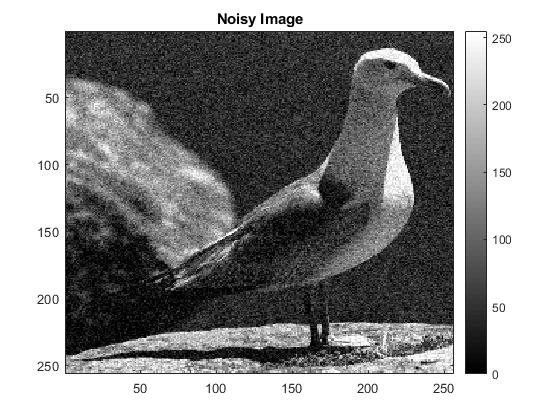
\includegraphics[width = 0.5\textwidth]{Images/Noisy.jpg}
		\caption{Image of a bird corrupted by noise}
		\label{noise}
	\end{figure}
\end{center}



\begin{figure}[h!]
\captionsetup[subfloat]{labelformat=empty}
\centering
\subfloat[]{
  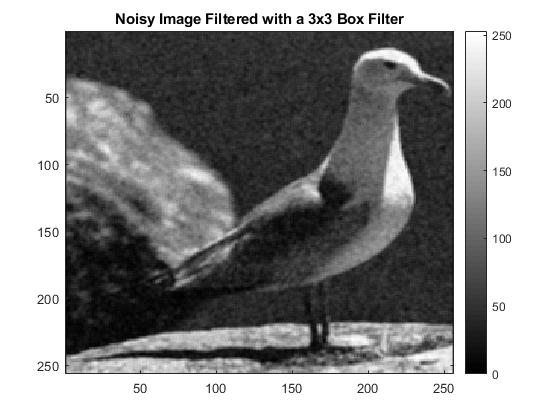
\includegraphics[width=50mm]{box3.jpg}
}
\subfloat[]{
  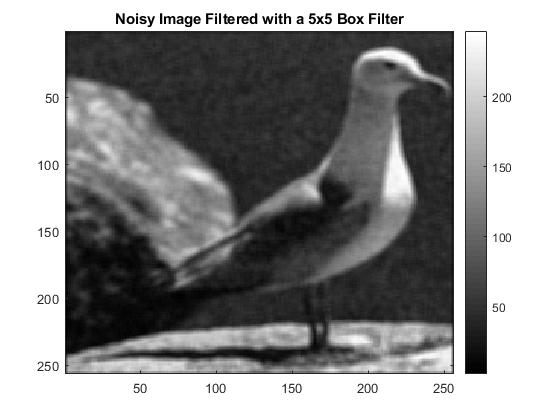
\includegraphics[width=50mm]{box5.jpg}
}
\hspace{0mm}
\subfloat[]{
  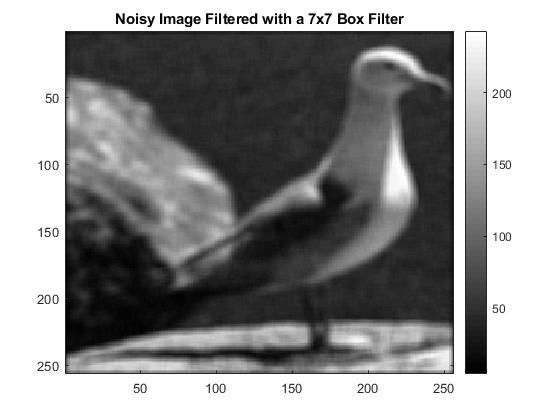
\includegraphics[width=50mm]{box7.jpg}
}
\subfloat[]{
  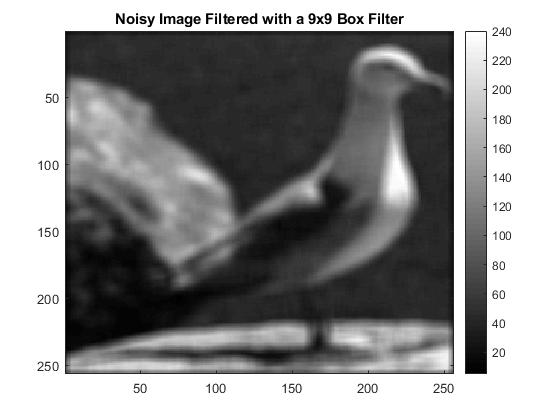
\includegraphics[width=50mm]{box9.jpg}
}
\caption{Box filtered images of the noisy bird image shown in fig. \ref{noise}.  Kernel sizes are top left: 3x3, top right: 5x5, bottom left: 7x7, and bottom right: 9x9}
\label{box}
\end{figure}

\begin{figure}[h!]
\captionsetup[subfloat]{labelformat=empty}
\centering
\subfloat[]{
  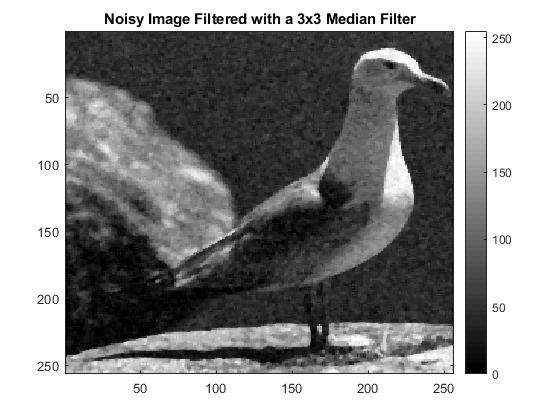
\includegraphics[width=50mm]{median3.jpg}
}
\subfloat[]{
  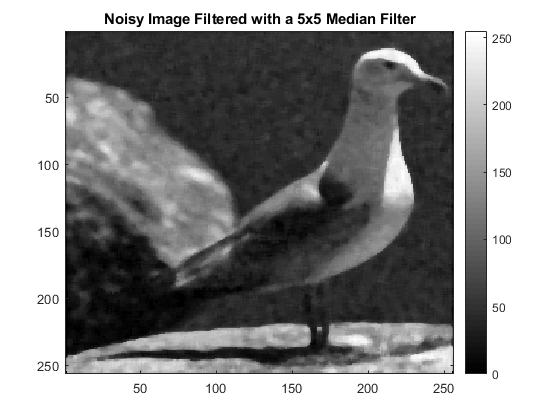
\includegraphics[width=50mm]{median5.jpg}
}
\hspace{0mm}
\subfloat[]{
  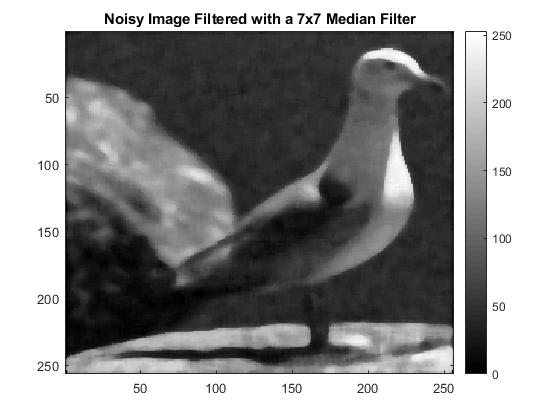
\includegraphics[width=50mm]{median7.jpg}
}
\subfloat[]{
  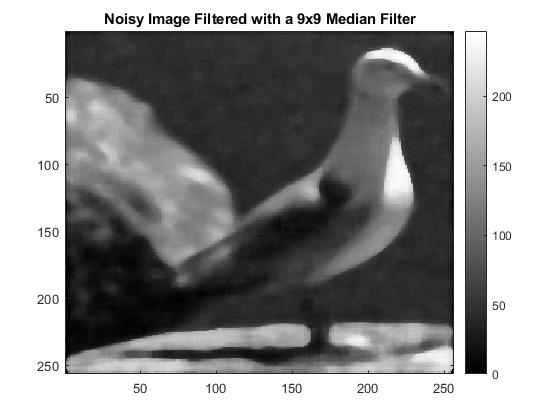
\includegraphics[width=50mm]{median9.jpg}
}
\caption{Median filtered images of the noisy bird image shown in fig. \ref{noise}.  Kernel sizes are top left: 3x3, top right: 5x5, bottom left: 7x7, and bottom right: 9x9}
\label{median}
\end{figure}

\noindent
From visual inspection of the filtered images, a few things can be observed.  First, the blurring effect of the filters is increased with increases in the kernel size, i.e. the 3x3 provides less blurring than the 9x9.  Next, for all kernel sizes, the averaging filter seems to do a better job of removing noise.  However, it also blurs the features more, therefore, reducing contrast.  A observed in the 7x7 and 9x9 filtered images, the median filter preserves contrast better than the box filter.  This aspect is especially noticed in the high intensity values on the head and breast of the bird. Additionally, the box filter is more affected by the zero padding.  This can be seen around the edges of the image, where pixel values were darkened.  A few more qualities can be noticed in the images.  One, the boundaries provided by the box filter are fairly rough or "jagged".  Two, the median filter's boundaries are more sharp, but overall, there is more noise in the images.  These two properties are inherent of the filter types and were, therefore, expected.

\section*{Part III Extra Credit}


\noindent
From the description of the kernels, the Gaussian kernel can be constructed as 
\begin{align*}
\bm{G} = 
\begin{bmatrix}
    0.025 & 0.108 & 0.025 \\
    0.108 & 0.469 & 0.108 \\
    0.025 & 0.108 & 0.025     
\end{bmatrix}
\end{align*}

and the Differentiating kernel can be defined as the outer product of the 1D kernels, providing 
\begin{align*}
\bm{D} = 
\begin{bmatrix}
    0.25 & 0 & -0.25 \\
    0 & 0 & 0 \\
    -0.25 & 0 & 0.25
\end{bmatrix}
\end{align*}

The convolution of these two kernels yields 

\begin{align*}
\bm{G}*\bm{D} = 
\begin{bmatrix}
    0.0063 & 0 & -0.0063 \\
    0 & 0 & 0 \\
    -0.0063 & 0 & 0.0063
\end{bmatrix}
\end{align*}

\noindent
This kernel is undesirable due to the fact that it's sharpening effect is greatly diminished.  Applying smoothing reduces the contrast in an image and blurs the features that we would like to enhance by sharpening.  So if we blur before sharpening, we are trying to enhance boundaries that have already been stretched out, providing visually unappealing results. \\



 
 \noindent 
 Accompanying code is provided in $mccurleyHW03.m$ and $myfilt.m$


\end{document}
